\documentclass[11pt, notitlepage]{article}

%package imports
\usepackage[T1]{fontenc}
\usepackage[letterpaper, margin=1in]{geometry}  %for letter-sized paper
\usepackage{setspace}              %double spacing
\usepackage{fancyhdr}              %header capability
\usepackage{graphicx}
\usepackage{booktabs}
\usepackage{amsmath}
\usepackage{amssymb}
\usepackage{amsthm}
\usepackage{wrapfig}

%page layout setup
\setlength{\headheight}{14.5pt}
\setlength{\headsep}{25pt}

%header setup
\pagestyle{fancyplain}
\fancyhf{}

\lhead{\fancyplain{}{\today}}                 %top left
\chead{\fancyplain{}{CPSC 121: Assignment 1}}                                 %top center
\rhead{\fancyplain{}{Calvin Cheng \& Brian Wu}}	                    %top right
\lfoot{\fancyplain{}{}}                                 %bottom left
\cfoot{\fancyplain{}{---\thepage---}}                   %bottom center
\rfoot{\fancyplain{}{}}                                 %bottom right

\renewcommand{\headrulewidth}{0pt}
\renewcommand{\footrulewidth}{0pt}

\renewcommand{\qedsymbol}{$\blacksquare$}

\newcommand{\unit}[1]{\;\textrm{#1}}
\newcommand*{\oldneg}{\mathord{\sim}}

\newcommand*\adjustwrapfigitem{\null\vskip-\baselineskip}

%document beginning
\begin{document}

%line spacing
\setstretch{1.075}

\begin{enumerate}

\item \begin{enumerate}

\item A $\sim$, or a NOT gate, can be simulated using only NAND gates by simply passing the same signal through the gate as shown below:
\begin{center}
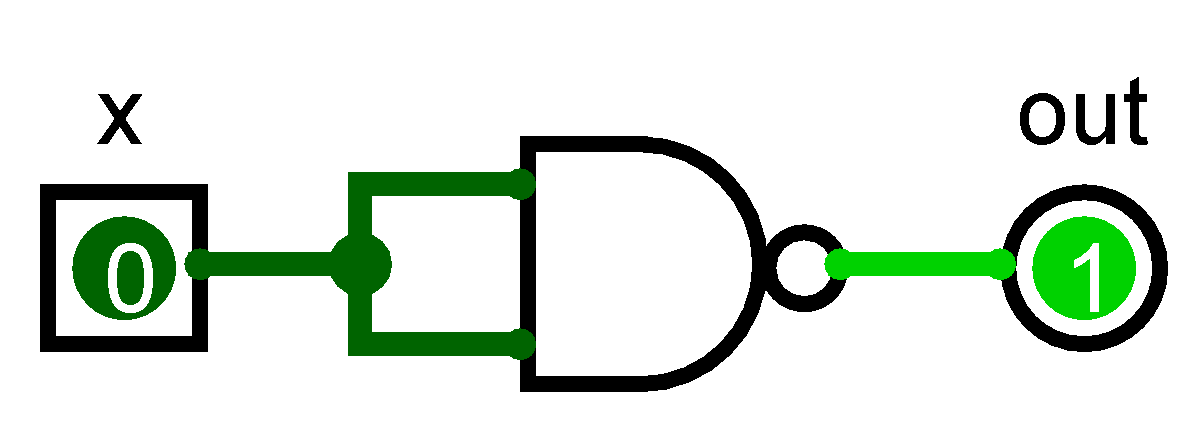
\includegraphics[scale=0.1]{1a}
\end{center}

\item An AND gate can be designed using only NAND gates given that $\oldneg (\oldneg (p \wedge q)) \equiv p \wedge q$:
\begin{center}
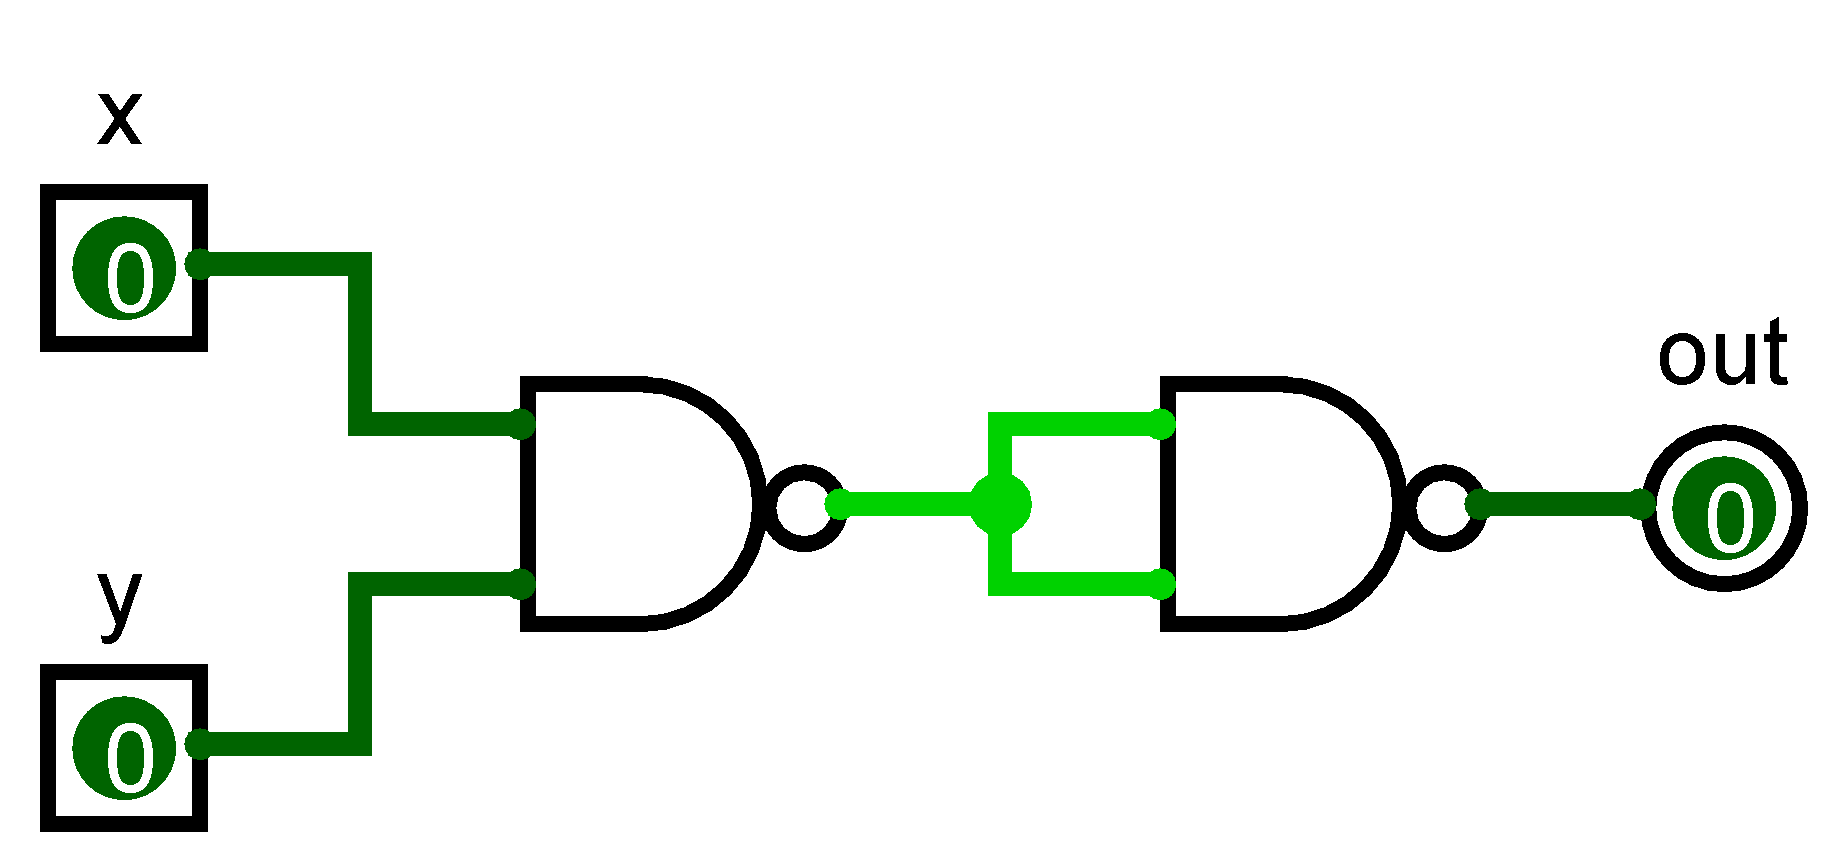
\includegraphics[scale=0.1]{1b}
\end{center}

\item Using de Morgan's law, we find that $\oldneg (\oldneg x \wedge \oldneg y) \equiv x \vee y$. Since we have the NOT and AND expressions from the previous two questions, we can derive the circuit for an OR gate as shown below:
\begin{center}
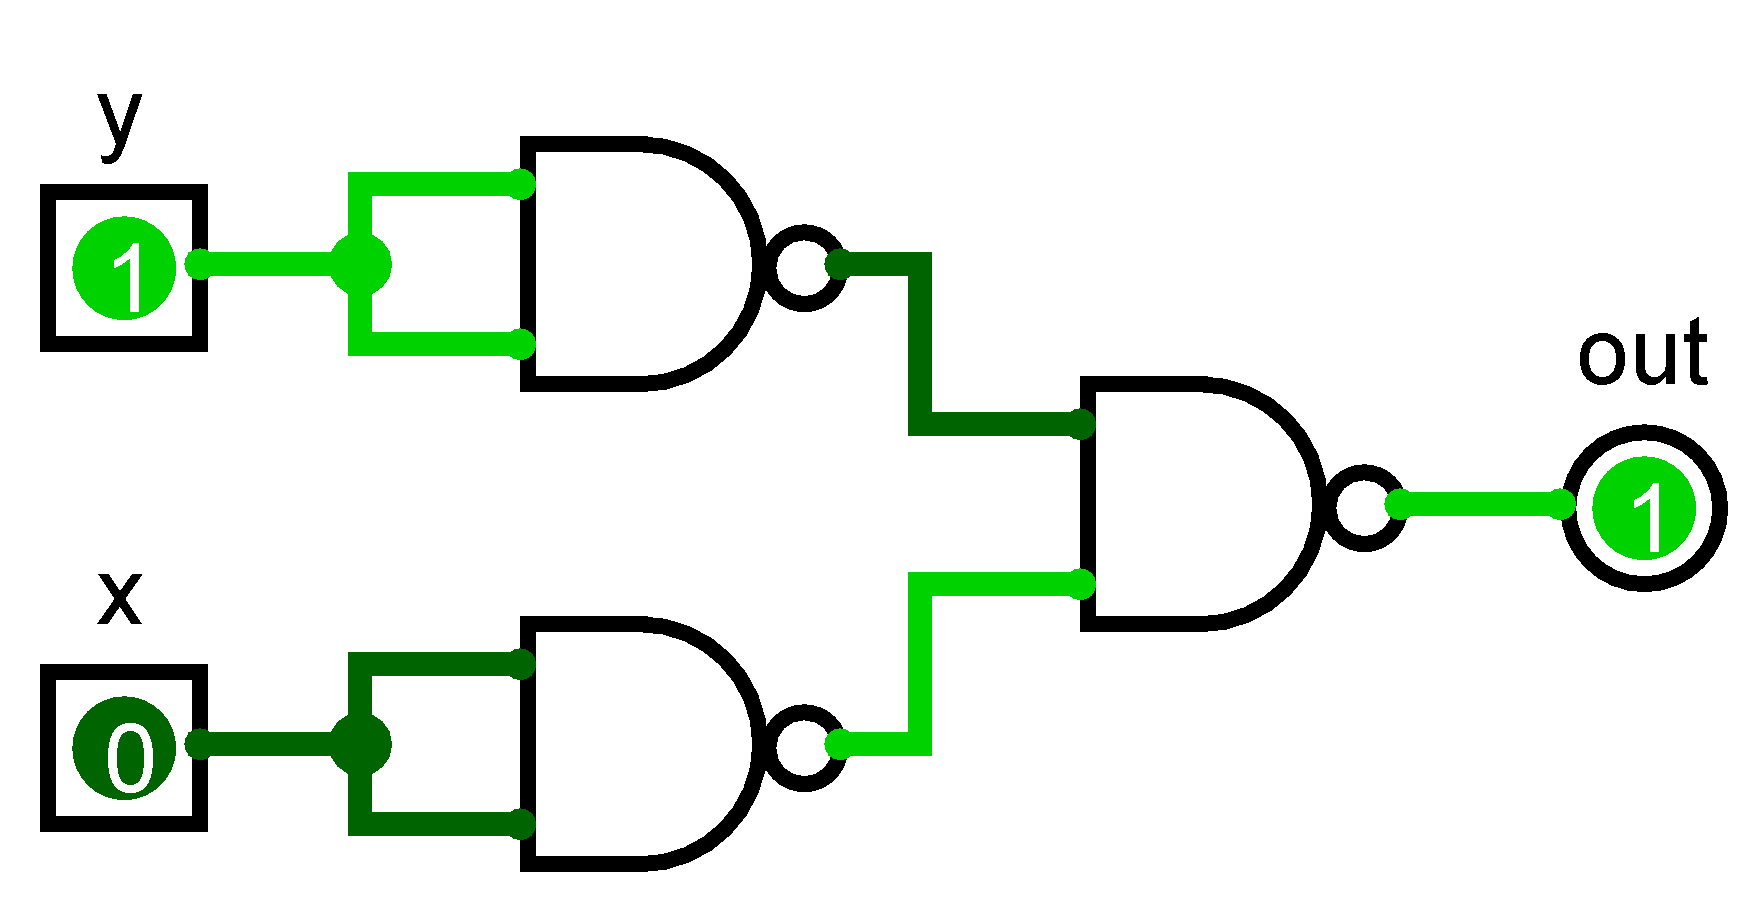
\includegraphics[scale=0.1]{1c}
\end{center}

\item From the first three questions, we find that NOT, AND, and OR gates can all be designed using only 2-input NAND gates. Given that all logical propositions are derived from a combination of these logic functions, we can then conclude that any number of atomic propositions can be implemented.

Another way to look at this is to recognize that all statements can be reduced to using the logic symbols $\sim$, $\wedge$, or $\vee$ only---since each of these operators can be represented using only 2-input NAND gates, it follows that all statements can be represented using only 2-input NAND gates.

\end{enumerate}

\item \begin{enumerate}

\item A valid logic formula is $(\oldneg p \wedge q) \vee (p \wedge\oldneg r)$. The truth table is shown below:
\begin{center}
\begin{tabular}{|ccc||cccc|c|c|}
	\toprule
	$p$ & $q$ & $r$ & $\oldneg p$ & $(\oldneg p \wedge q)$ & $\oldneg r$ & $(p \wedge \oldneg r)$ & $(\oldneg p \wedge q) \vee (p \wedge \oldneg r)$ & $s$\\
	\midrule
	F & F & F & T & F & T & F & F & F\\
	F & F & T & T & F & F & F & F & F\\
	F & T & F & T & T & T & F & T & T\\
	F & T & T & T & T & F & F & T & T\\
	T & F & F & F & F & T & T & T & T\\
	T & F & T & F & F & F & T & F & F\\
	T & T & F & F & F & T & F & T & T\\
	T & T & T & F & F& F  & F & F & F\\
	\bottomrule
\end{tabular}
\end{center}

\item The circuit that represents the logic formula above is shown below:
\begin{center}
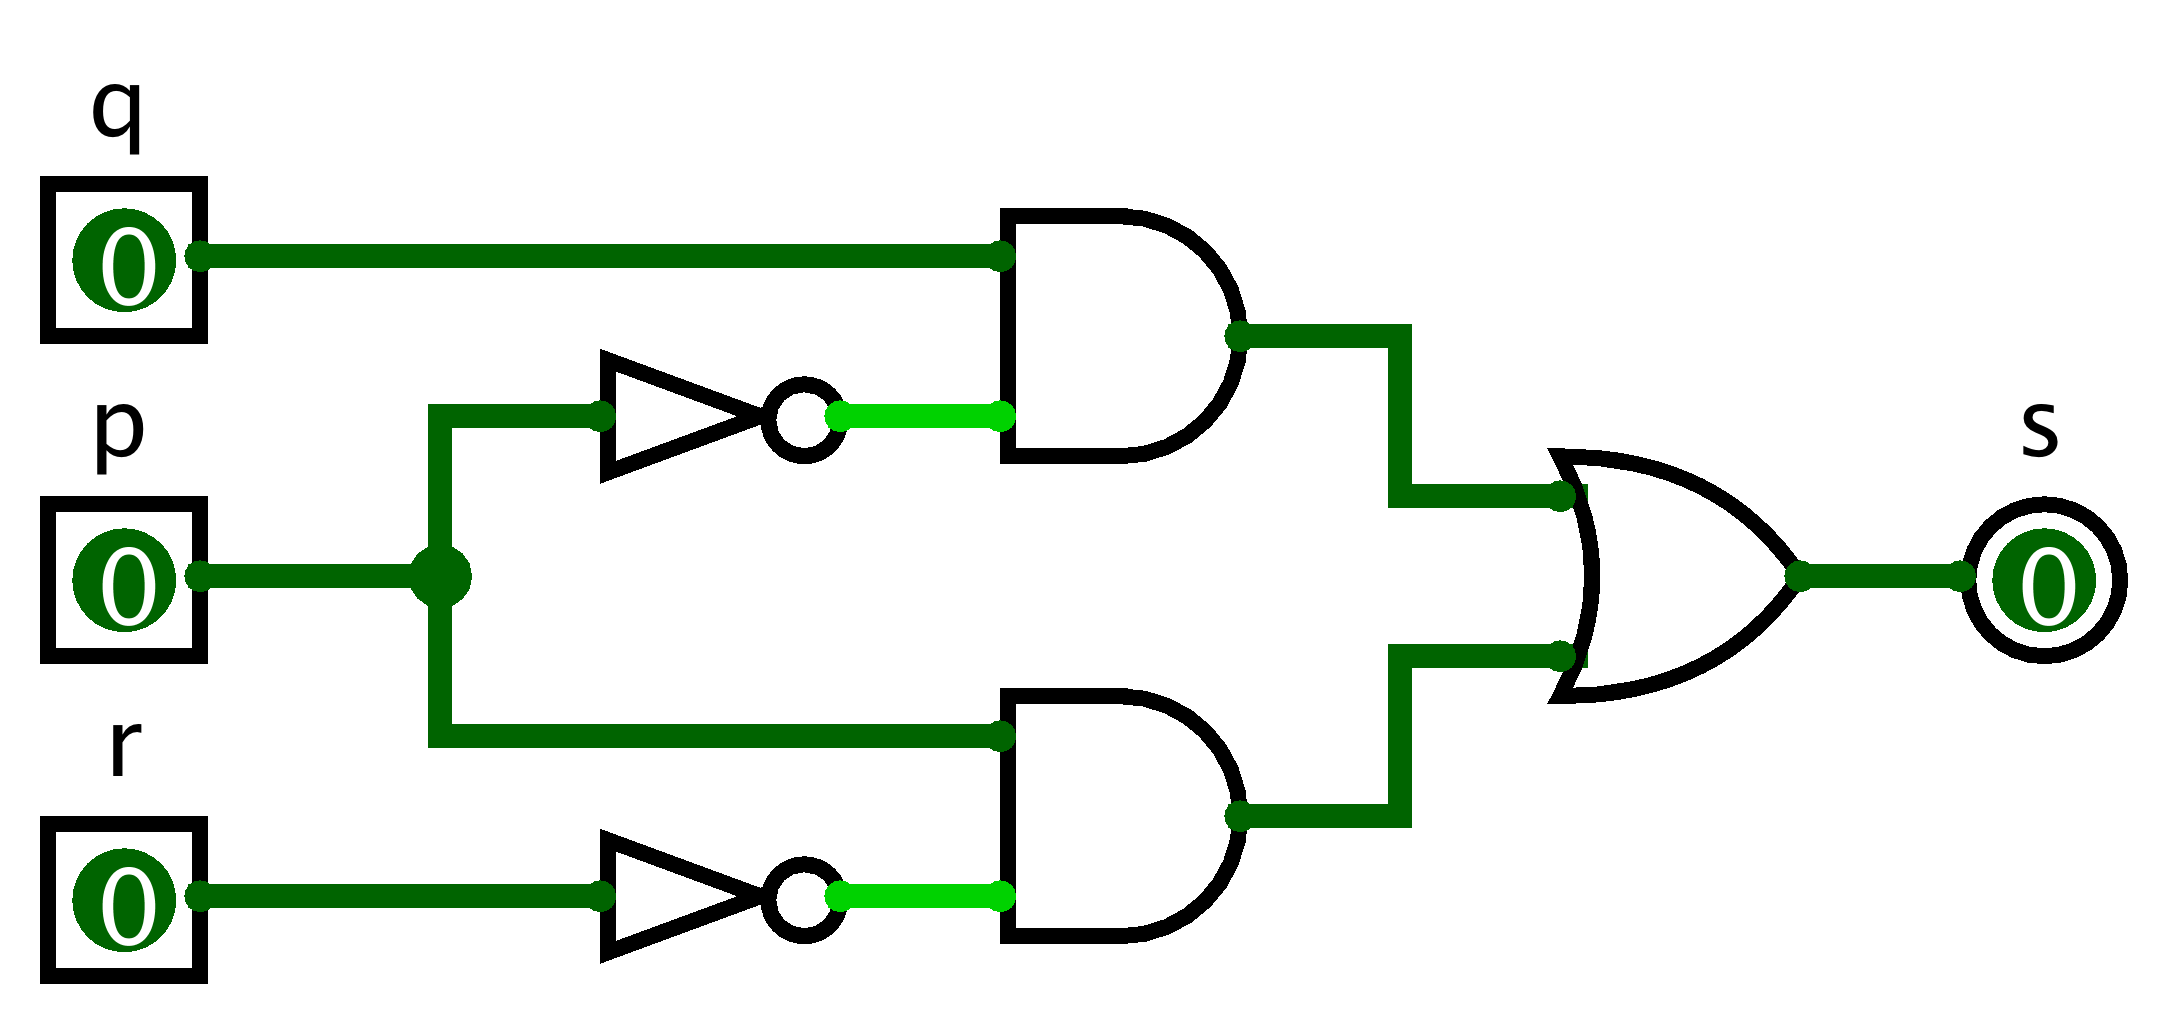
\includegraphics[scale=0.1]{2b}
\end{center}
\end{enumerate}

\item $(a)$ is logically equivalent to $(c)$. Below is the proof that $(c \vee a) \to (c \vee b) \equiv (c \vee (a \to b))$:

\textit{Proof.}
\vspace{-25pt}
\begin{align*}
 	\textrm{LHS} &\equiv (c \vee a) \to (c \vee b)\\
 		&\equiv \oldneg (c \vee a) \vee (c \vee b) && \textrm{[IMP]}\\
 		&\equiv (\oldneg c \wedge \oldneg a) \vee (c \vee b) && \textrm{[DM]}\\
 		&\equiv ((\oldneg c \wedge \oldneg a) \vee c) \vee b && \textrm{[ASS]}\\
 		&\equiv ((\oldneg c \vee c) \wedge (\oldneg a \vee c)) \vee b && \textrm{[DIST]}\\
 		&\equiv (T \wedge (\oldneg a \vee c)) \vee b && \textrm{[NEG]}\\
 		&\equiv (\oldneg a \vee c) \vee b && \textrm{[I]}\\
 		&\equiv (c \vee \oldneg a) \vee b && \textrm{[COM]}\\
 		&\equiv c \vee (\oldneg a \vee b) && \textrm{[ASS]}\\
 		&\equiv c \vee (a \to b) && \textrm{[IMP]}\\
 		&\equiv \textrm{RHS}\\
 		&\therefore (c \vee a) \to (c \vee b) \equiv (c \vee (a \to b)) && \blacksquare
\end{align*}

$(b)$ is logically equivalent to $(e)$. By translating the circuit diagram in $(e)$ into the logic statement $\oldneg ((a \oplus b) \vee (a \vee \oldneg b))$, we can prove that $\oldneg ((a \oplus b) \vee (a \vee \oldneg b)) \equiv \oldneg a \vee b$:

\textit{Proof.}
\vspace{-25pt}
\begin{align*}
 	\textrm{LHS} &\equiv \oldneg ((a \oplus b) \wedge (a \vee \oldneg b))\\
 		&\equiv \oldneg (((a \vee b) \wedge \oldneg (a \wedge b)) \wedge (a \vee \oldneg b)) && \textrm{[XOR]}\\
 		&\equiv \oldneg (((a \vee b) \wedge (a \vee \oldneg b)) \wedge \oldneg (a \wedge b)) && \textrm{[COM]}\\
 		&\equiv \oldneg ((a \wedge (b \vee \oldneg b)) \wedge \oldneg (a \wedge b)) && \textrm{[DIST]}\\
 		&\equiv \oldneg ((a \wedge T) \wedge \oldneg (a \wedge b)) && \textrm{[NEG]}\\
 		&\equiv \oldneg (a \wedge \oldneg (a \wedge b)) && \textrm{[I]}\\
 		&\equiv \oldneg a \vee \oldneg (\oldneg (a \wedge b)) && \textrm{[DM]}\\
 		&\equiv \oldneg a \vee (a \wedge b) && \textrm{[DNEG]}\\
 		&\equiv (\oldneg a \vee a) \wedge (\oldneg a \vee b) && \textrm{[DIST]}\\
 		&\equiv T \wedge (\oldneg a \vee b) && \textrm{[NEG]}\\
 		&\equiv \oldneg a \vee b && \textrm{[I]}\\
 		&\equiv \textrm{RHS}\\
 		&\therefore \oldneg ((a \oplus b) \vee (a \vee \oldneg b)) \equiv \oldneg a \vee b && \blacksquare
\end{align*}

$(d)$ is logically equivalent to $(f)$. By translating the circuit in $(f)$ into the logic statement $\oldneg (a \wedge \oldneg c) \vee \oldneg (b \vee c)$, we can prove that $(a \wedge (b \vee c)) \to (a \wedge c) \equiv \oldneg (a \wedge \oldneg c) \vee \oldneg (b \vee c)$:

\textit{Proof.}
\vspace{-25pt}
\begin{align*}
 	\textrm{LHS} &\equiv (a \wedge (b \vee c)) \to (a \wedge c)\\
 		&\equiv \oldneg (a \wedge (b \vee c)) \vee (a \wedge c) && \textrm{[IMP]}\\
 		&\equiv \oldneg a \vee \oldneg (b \vee c) \vee (a \wedge c) && \textrm{[DM]}\\
 		&\equiv \oldneg a \vee (\oldneg b \wedge \oldneg c) \vee (a \wedge c) && \textrm{[DM]}\\
 		&\equiv \oldneg a \vee (a \wedge c) \vee (\oldneg b \wedge \oldneg c) && \textrm{[COM]}\\
 		&\equiv ((\oldneg a \vee a) \wedge (\oldneg a \vee c)) \vee (\oldneg b \wedge \oldneg c) && \textrm{[DIST]}\\
 		&\equiv (T \wedge (\oldneg a \vee c)) \vee (\oldneg b \wedge \oldneg c) && \textrm{[NEG]}\\
 		&\equiv (\oldneg a \vee c) \vee (\oldneg b \wedge \oldneg c) && \textrm{[I]}\\
 		&\equiv \oldneg(a \wedge \oldneg c) \vee \oldneg (b \vee c) && \textrm{[DM]}\\
 		&\equiv \textrm{RHS}\\
 		&\therefore (a \wedge (b \vee c)) \to (a \wedge c) \equiv \oldneg (a \wedge \oldneg c) \vee \oldneg (b \vee c) && \blacksquare
\end{align*}

\item \begin{enumerate}

\item\parbox[t]{\textwidth}{
	\adjustwrapfigitem
        \begin{wraptable}{r}{2in}
        \vspace{-12pt}
	\begin{tabular}{|ccc||c|}
	\toprule
	$a$ & $b$ & $c$ & out\\
	\midrule
	F & F & F & F\\
	F & F & T & F\\
	F & T & F & F\\
	\textbf{F} & \textbf{T} & \textbf{T} & \textbf{T}\\
	T & F & F & F\\
	\textbf{T} & \textbf{F} & \textbf{T} & \textbf{T}\\
	\textbf{T} & \textbf{T} & \textbf{F} & \textbf{T}\\
	\textbf{T} & \textbf{T} & \textbf{T} & \textbf{T}\\
	\bottomrule
	\end{tabular}
	\end{wraptable}
       The formula for this problem is $(a \wedge b) \vee (a \wedge c) \vee (b \wedge c)$. This formula was determined by constructing the truth table, as shown to the right. The rows where the output is true are shown in bold. Since the output is true if at least two of the inputs are true, one can simply formulate an expression for the combinations, and combine each case with an OR expression. We also discover that the final row of the table, where all three inputs are true, is redundant given the first three cases, as all three inputs cannot be true without causing one of the prior cases to evaluate to true. Therefore, a valid logic formula that returns the same value as that of the majority of the three inputs is $(a \wedge b) \vee (a \wedge c) \vee (b \wedge c)$.}\\

\item A valid circuit that is equivalent to the truth table and logic expression determined in the previous question is shown below:
\begin {center}
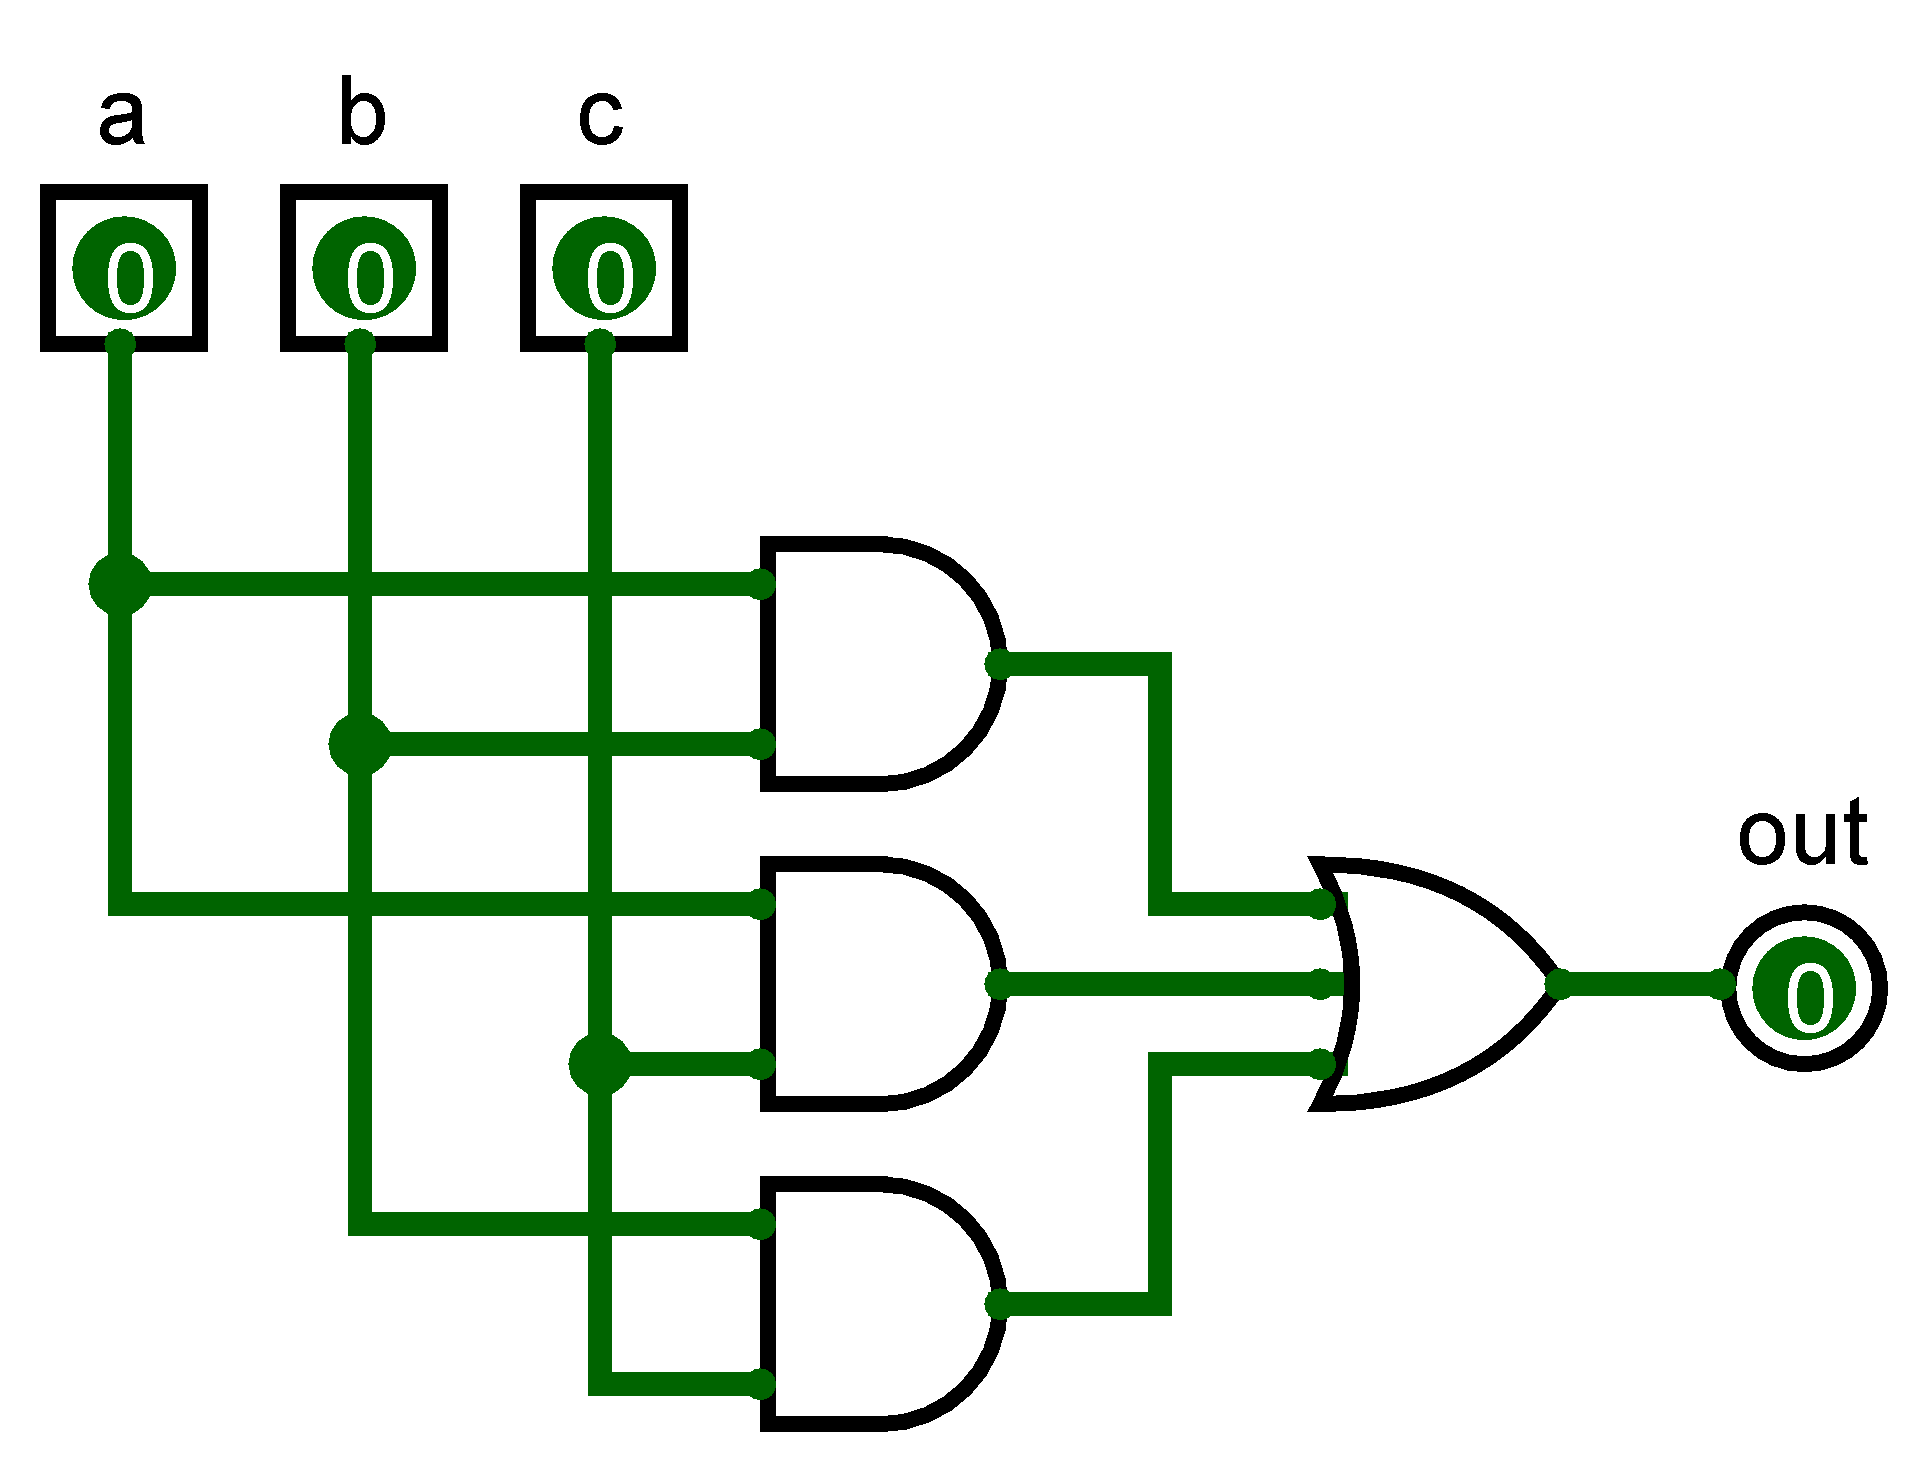
\includegraphics[scale=0.13]{4b}
\end{center}

\end{enumerate}

\item If Portia's boyfriend would like to marry Portia, he should choose the silver box.
\begin{proof}
Since only one of the three statements is true, let us evaluate each of the three cases individually. Let $g$, $s$, and $l$ represent the cases where the ring is in the gold, silver, and lead boxes, respectively.

First, we assume that the statement on the gold box is true. This would mean that the ring is in the gold box, and that neither is the ring not in the silver box nor is the ring not in the gold box. Symbolically:
\begin{align*}
	g \wedge \oldneg (\oldneg s) \wedge \oldneg(\oldneg g) &\equiv g \wedge s \wedge g &&\textrm{[DNEG]}\\
	&\equiv g \wedge g \wedge s &&\textrm{[COM]}\\
	&\equiv g \wedge s &&\textrm{[ID]}
\end{align*}
After simplification, we see that the only case in which this expression can be true is if the ring is in both the gold and silver boxes. As this is clearly not the case, the statement on the gold box must be false.

Next, let us assume that the statement on the silver box is true. This would mean that the ring is not in the gold box, that the ring is not in the silver box, and that it is not the case that the ring is not in the gold box. Symbolically:
\begin{align*}
	\oldneg g \wedge \oldneg s \wedge \oldneg(\oldneg g) &\equiv \oldneg g \wedge \oldneg s \wedge g &&\textrm{[DNEG]}\\
	&\equiv \oldneg g \wedge g \wedge \oldneg s &&\textrm{[COM]}\\
	&\equiv F \wedge \oldneg s &&\textrm{[NEG]}\\
	&\equiv F &&\textrm{[UB]}
\end{align*}
After simplification, we clearly see that this expression is a contradiction---it can never be true. Therefore, the statement on the silver box must be false.

Given that the statements on the first two boxes were impossible, the statement on the lead box must be true. Nonetheless, this can be shown more rigorously, as well. If the statement on the lead box is true, it means that it is not the case that the ring is in the gold box, that the ring is in the silver box, and that the ring is not in the gold box. Symbolically:
\begin{align*}
	\oldneg g \wedge \oldneg (\oldneg s) \wedge \oldneg g &\equiv \oldneg g \wedge s \wedge \oldneg g &&\textrm{[DNEG]}\\
	&\equiv \oldneg g \wedge \oldneg g \wedge s &&\textrm{[COM]}\\
	&\equiv \oldneg g \wedge s &&\textrm{[ID]}
\end{align*}
The only case in which this expression is true is if the ring is in the silver box, and not in the gold box. Therefore, the statement on the lead box is valid, and the engagement ring must be found inside the silver box. As a result, Portia's boyfriend should choose the silver box. \qedhere

\end{proof}

\end{enumerate}


\end{document}